% =====================================================================
% Relatório 4 -- Encoder e controle PID (12 pontos).
% Estrutura do enunciado (Seção 8): introdução, montagem, modelo do
% encoder, malha aberta, filtros, PID, resultados, discussão, conclusão.
% Todos os números vêm de TP4/calculos.md e dos CSVs em TP4/dados/.
% Marcações em vermelho (\pendente) são o que ainda precisa ser
% confirmado pela equipe antes da entrega: grep -n 'pendente' relatorio.tex
% =====================================================================

\documentclass[11pt,a4paper]{article}

\usepackage[utf8]{inputenc}
\usepackage[T1]{fontenc}
\usepackage[brazil]{babel}
\usepackage{lmodern}
\usepackage[margin=2.3cm]{geometry}
\usepackage{graphicx}
\usepackage{amsmath}
\usepackage{amssymb}
\usepackage{booktabs}
\usepackage{array}
\usepackage{tabularx}
\usepackage{float}
\usepackage{caption}
\usepackage{subcaption}
\usepackage{enumitem}
\usepackage{xcolor}
\usepackage{indentfirst}
\usepackage{placeins}
\usepackage[hyphens]{url}
\usepackage[hidelinks]{hyperref}

\graphicspath{{figuras/}}

\captionsetup{font=small,skip=4pt}
\newcolumntype{L}{>{\raggedright\arraybackslash}X}

\renewcommand{\topfraction}{0.92}
\renewcommand{\bottomfraction}{0.85}
\renewcommand{\textfraction}{0.06}
\renewcommand{\floatpagefraction}{0.75}
\setcounter{topnumber}{3}
\setcounter{bottomnumber}{2}
\setcounter{totalnumber}{5}
\setlength{\parskip}{0.15em}

\newcommand{\pendente}[1]{\textcolor{red}{\textbf{[FALTA:} #1\textbf{]}}}
\newcommand{\unid}[1]{\,\mathrm{#1}}

\title{\textbf{Relatório 4: Encoder e controle PID de velocidade}\\
[0.4em]
\large Medida de distância e velocidade de uma roda com encoder e malha fechada sobre um servo de giro contínuo}

\author{
Vinicius Trindade Dias Abel \\
Guilherme Buxbaum Marinho Guerra \\
Thiago Henrique Silva de Almeida \\
Rafael Santos Oliveira \\[0.8em]
\small Departamento de Ciência da Computação \\
\small Universidade Federal de Minas Gerais \\
\small Projeto de Sistemas Robóticos, Prof. Paulo Rezeck
}

\date{Belo Horizonte, novembro de 2026}

\begin{document}

\maketitle

\begin{abstract}
\noindent
Este relatório descreve a montagem de uma roda acionada por um servo MG90S de giro contínuo, com um encoder mecânico acoplado por engrenagem, e o controle da velocidade dela com um PID rodando numa Arduino Mega. Medidos na própria bancada, o diâmetro da roda é $D = 43{,}40\unid{mm}$ (paquímetro) e o encoder produz $N = 287{,}3 \pm 0{,}6$ ticks por volta, em X4, o que dá $k = 0{,}4746 \pm 0{,}0011\unid{mm/tick}$. Com período de leitura de $50\unid{ms}$ (medido, $50{,}000\unid{ms}$ com desvio de $9\unid{\mu s}$), a velocidade anda em degraus de $9{,}5\unid{mm/s}$. A busca do neutro na bancada deu $1495\unid{\mu s}$ em duas corridas, com banda morta de cerca de $60\unid{\mu s}$ e salto de $0$ a $\approx 80\unid{mm/s}$ na saída dela. Dos dois filtros comparados num degrau, a média móvel de 5 amostras e o passa-baixa com $\alpha = 0{,}3$, foi escolhida a média móvel, que corta o ruído em cerca de três vezes e assenta em $0{,}32\unid{s}$. Os ganhos finais, $k_p = 3\unid{\mu s/(mm/s)}$, $k_i = 8\unid{\mu s/(mm/s)/s}$ e $k_d = 0$, deram erro de regime abaixo de $0{,}6\,\%$ em cinco patamares de $100$ a $160\unid{mm/s}$ e inverteram o sentido de $+120$ a $-120\unid{mm/s}$ em cerca de $0{,}55\unid{s}$. A correção limitada a $\pm 250\unid{\mu s}$ impede a malha de passar de $\approx 165\unid{mm/s}$, embora a curva aberta chegue a $272\unid{mm/s}$. Em três voltas a $120\unid{mm/s}$, a roda andou $414{,}8\unid{mm}$ contra $409{,}0\unid{mm}$ esperados, $1{,}4\,\%$ a mais.
\end{abstract}

\section{Introdução}

Um servo de giro contínuo recebe uma largura de pulso e gira com uma velocidade que depende dela, mas não informa quanto a roda andou nem com que velocidade. Para saber isso, é preciso medir: um encoder conta ticks, e uma constante em milímetros por tick converte a contagem em distância e em velocidade. Com a velocidade medida, o pulso passa a ser corrigido por uma malha fechada até a roda acompanhar a velocidade pedida.

O que a equipe entregou neste trabalho foi:
\begin{itemize}[nosep]
  \item a montagem da transmissão (servo, roda e encoder), com fotos;
  \item as medidas de $D$ e de $N$ e a constante $k$ em mm/tick, com sua incerteza e o degrau de quantização da velocidade;
  \item o neutro do servo, procurado na bancada, e a curva do pulso contra a velocidade em malha aberta, com banda morta, saturação e assimetria;
  \item a comparação de dois filtros da velocidade num mesmo degrau e a escolha de um;
  \item o PID, a sintonia (tabela de cinco tentativas) e os três ensaios pedidos: cinco patamares, inversão de sentido e distância.
\end{itemize}
O código, os registros em CSV e os \textit{scripts} que refazem os gráficos estão no repositório da equipe\footnote{\url{https://github.com/rafaelos134/Sistemas_Roboticos_2026}, ramo \texttt{tp4-firmware-controle}, pasta \texttt{TP4/}.}.

\section{Montagem}

\subsection{As duas transmissões}

A peça impressa traz um lado do chassi, com lugar para a roda, o servo e o encoder. Há duas relações mecânicas. O pinhão do servo aciona a engrenagem da roda, e uma segunda engrenagem, solidária à roda, aciona o encoder (Figura~\ref{fig:engrenagens}). Por isso a grandeza que importa é o número de ticks que o encoder produz numa volta da \emph{roda}, e não o do disco do encoder sozinho. A decodificação é feita em X4 (subida e descida dos canais A e B), com a biblioteca \texttt{Encoder} de Paul Stoffregen~\cite{encoder}.

\begin{figure}[htbp]
  \centering
  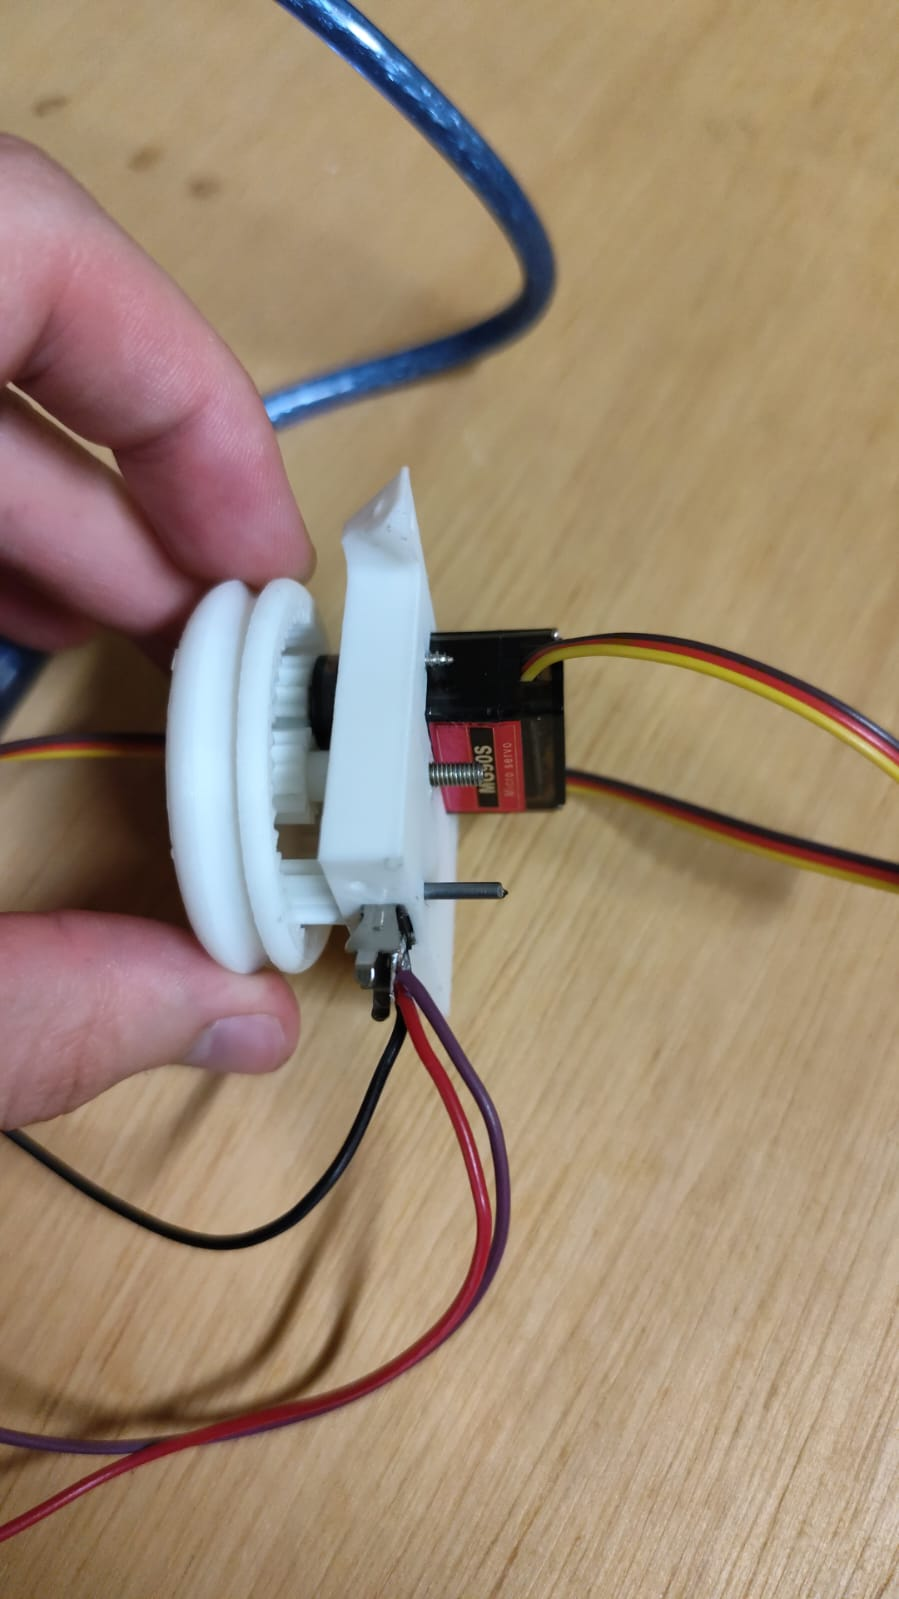
\includegraphics[height=7.5cm]{engrengans.jpg}
  \caption{Transmissão engrenada, vista pelo lado das engrenagens. À direita, o servo MG90S preso ao chassi impresso. No centro, a roda com a engrenagem solidária que aciona o encoder, na parte de baixo, de onde saem os três fios do encoder (GND, A e B).}
  \label{fig:engrenagens}
\end{figure}

\subsection{Ligações}

O servo está no header Servo1 do shield de motores (``Motor Driver V2.0'', um clone do L293D), com o sinal no pino D10 da Mega. O enunciado indica o D9. Um teste de sanidade confirmou que o servo gira com o sinal no D10 (o D9 não foi testado): pulso de $2000\unid{\mu s}$ dá ticks crescentes e de $1000\unid{\mu s}$ dá ticks decrescentes. O encoder é um modelo mecânico de três pinos, com o comum no GND e os canais A e B nos pinos de interrupção D2 e D3, com os \textit{pull-ups} internos ligados e nada no 5\,V. As ligações estão nas Figuras~\ref{fig:mega}\subref{fig:mega1} e~\ref{fig:mega}\subref{fig:mega2}. O shield aparece com uma fonte externa no borne de potência \pendente{tensão da fonte e se ela estava ligada em todos os ensaios; no relatório, declarar a alimentação do servo}.

\begin{figure}[htbp]
  \centering
  \begin{subfigure}[b]{0.36\linewidth}
    \centering
    \includegraphics[height=7.2cm]{"arduino e roda.jpg"}
    \caption{Conjunto: Mega com o shield, cabo USB, fonte externa e o chassi com a roda.}
    \label{fig:mega1}
  \end{subfigure}\hfill
  \begin{subfigure}[b]{0.60\linewidth}
    \centering
    \includegraphics[height=7.2cm]{"arduino e roda 2.jpg"}
    \caption{Detalhe: o cabo do servo no header do shield e os fios do encoder indo aos pinos 2 e 3 e ao GND.}
    \label{fig:mega2}
  \end{subfigure}
  \caption{Ligação do servo e do encoder na Arduino Mega 2560 com o shield de motores.}
  \label{fig:mega}
\end{figure}

\subsection{Servos usados}

A bancada passou por três servos. Um primeiro MG90S deu erro, foi trocado por um SG90, que também deu erro, e depois por um segundo MG90S novo, o atual, com a mesma roda, o mesmo encoder e a mesma transmissão. As medidas de $N$, de $D$ e de $k$ (Seção~\ref{sec:encoder}) não dependem do servo e foram feitas com o primeiro, e valem para os outros. \textbf{Todas as medidas a partir da Seção~\ref{sec:aberta} (neutro, curva aberta, filtros, sintonia e ensaios) são do MG90S novo.} Uma primeira busca do neutro, com um servo anterior, deu $1485\unid{\mu s}$ e é descartada.

\section{Modelo do encoder}
\label{sec:encoder}

Os símbolos são os do enunciado: $D$ é o diâmetro da roda na banda de contato, $N$ é o número de ticks por volta da roda, e
\begin{equation}
  k = \frac{\pi D}{N}, \qquad s = k \cdot \text{ticks}, \qquad v = \frac{\Delta s}{\Delta t}.
\end{equation}

\subsection{Ticks por volta, $N$}

$N$ foi medido girando a roda à mão, uma volta inteira de cada vez, com o contador zerado antes de cada volta, nos dois sentidos, com a biblioteca \texttt{Encoder} em X4. Duas contagens anteriores foram descartadas: uma em que o código girava o motor até um número de ticks (cerca de 366, porque o servo passa do ponto depois de parar), e outra com rotinas de interrupção próprias (média de $429 \pm 5{,}5$, com faixa de 403 a 465, espalhamento grande demais). A medida adotada tem 10 voltas em cada sentido (Tabela~\ref{tab:N}).

\begin{table}[htbp]
\centering
\caption{Ticks por volta da roda, em X4, em módulo. Vinte voltas à mão, com a biblioteca \texttt{Encoder}.}
\label{tab:N}
\begin{tabular}{lcccccc}
\toprule
Sentido & $n$ & Média & Mediana & Desvio $s$ & $s/\sqrt{n}$ & Faixa \\
\midrule
Positivo & 10 & 286,4 & 287,0 & 2,32 & 0,73 & 281 a 289 \\
Negativo & 10 & 288,2 & 288,5 & 2,53 & 0,80 & 283 a 291 \\
Todas    & 20 & \textbf{287,3} & 288,0 & 2,54 & 0,57 & 281 a 291 \\
\bottomrule
\end{tabular}
\end{table}

Os dois sentidos dão módulos próximos. A diferença das médias é de $1{,}8$ ticks, com erro padrão de $\sqrt{0{,}73^2 + 0{,}80^2} = 1{,}09$ ticks, o que dá $t = 1{,}66$ no teste de Welch (cerca de 18 graus de liberdade, $p \approx 0{,}11$). A diferença não é significativa a 5\,\%, então os dois sentidos são tratados como iguais e se usa um único valor,
\begin{equation}
  N = 287{,}3 \pm 0{,}6 \ \text{ticks/volta},
\end{equation}
compatível com os $288$ ticks da bancada de referência (48 pulsos do encoder e redução de 1:6): a diferença de $0{,}7$ tick é $1{,}3$ erro padrão. Com a biblioteca, o desvio caiu de 20 para $2{,}5$ ticks em relação às rotinas próprias.

\subsection{Diâmetro e constante $k$}

$D$ foi medido com \textbf{paquímetro}, na roda montada, na banda que toca o chão: $D = 43{,}40\unid{mm}$ (resolução assumida de $\pm 0{,}05\unid{mm}$). Uma medida pelo perímetro marcado sobre papel (46\,mm) foi descartada, porque tinha incerteza de cerca de $\pm 1\unid{mm}$ no perímetro. Então
\begin{align}
  \pi D &= 136{,}35\unid{mm}, \\
  k &= \frac{136{,}35}{287{,}3} = 0{,}4746\unid{mm/tick} \quad (1/k = 2{,}107\ \text{tick/mm}).
\end{align}
A incerteza vem de $N$ ($\pm 0{,}0009$) e de $D$ ($\pm 0{,}0005$), e combinadas em quadratura dão $k = 0{,}4746 \pm 0{,}0011\unid{mm/tick}$ ($0{,}2\,\%$). O $k$ de referência, $\pi \cdot 49{,}2/288 = 0{,}537\unid{mm/tick}$, é $12\,\%$ maior, e a diferença vem do diâmetro: a roda da bancada tem $11{,}8\,\%$ menos diâmetro que a de referência.

\subsection{Degrau de quantização}

A velocidade medida anda em degraus de $k/\Delta t$, porque numa janela só cabem ticks inteiros. O código lê o encoder a cada $50\unid{ms}$, com o instante da leitura tomado de \texttt{micros()}, e o $\Delta t$ da conta é o intervalo medido entre as duas leituras. No registro da curva aberta (1259 amostras, motor girando), o $\Delta t$ ficou em $50{,}000\unid{ms}$, com desvio de $9{,}2\unid{\mu s}$ e faixa de $49860$ a $50140\unid{\mu s}$ ($\pm 0{,}3\,\%$), então o degrau é
\begin{equation}
  \frac{k}{\Delta t} = \frac{0{,}4746}{0{,}050} = 9{,}5\unid{mm/s}.
\end{equation}
Para $20\unid{ms}$ seria $23{,}7\unid{mm/s}$, e para $100\unid{ms}$, $4{,}7\unid{mm/s}$. Em baixa velocidade o efeito é grande: a $30\unid{mm/s}$ caberiam só $3{,}2$ ticks na janela de $50\unid{ms}$ ($1{,}5\unid{mm}/0{,}4746$), e um tick a mais ou a menos mudaria a leitura em $32\,\%$. É isso que obriga a filtrar a velocidade (Seção~\ref{sec:filtros}). Mesmo na menor velocidade que a malha segura, $\approx 80\unid{mm/s}$, entram só $8{,}4$ ticks por janela, e a velocidade bruta ainda varia ao redor de $\pm 10\unid{mm/s}$.

\section{Malha aberta: pulso e velocidade}
\label{sec:aberta}

\subsection{Neutro medido}

O neutro é o pulso em que a roda para, e cada servo tem o seu. Ele foi procurado na bancada, em passos de $10\unid{\mu s}$, com o firmware aplicando cada pulso por $5\unid{s}$, descartando o primeiro segundo (transitório) e contando os ticks nos $4\unid{s}$ seguintes. A roda foi considerada parada com no máximo 2 ticks em $4\unid{s}$. A busca de 1300 a $1700\unid{\mu s}$ achou:
\begin{itemize}[nosep]
  \item roda girando para trás até $1460\unid{\mu s}$ ($-75{,}2\unid{mm/s}$);
  \item roda parada de $1470$ a $1520\unid{\mu s}$;
  \item roda girando para a frente a partir de $1530\unid{\mu s}$ ($+80{,}1\unid{mm/s}$).
\end{itemize}
O neutro é o ponto médio da faixa parada, $(1470 + 1520)/2 = \mathbf{1495\unid{\mu s}}$. Uma segunda corrida do mesmo comando deu a mesma faixa parada, de 1470 a $1520\unid{\mu s}$, e de novo $1495\unid{\mu s}$, então o neutro se repete. A banda morta fica em $1465$ a $1525\unid{\mu s}$, cerca de $60\unid{\mu s}$, e é a da bancada inteira (servo, transmissão e roda) vista pelo encoder: ela inclui, além da banda do circuito do servo, o atrito estático das engrenagens e da roda. O neutro não pode ser escrito como $1500\unid{\mu s}$ por convenção: a busca deu $1495\unid{\mu s}$, e o neutro do servo anterior era $1485\unid{\mu s}$.

\subsection{Curva pulso $\times$ velocidade}

Com o neutro fixado, o firmware varreu os pulsos de 1000 a $2000\unid{\mu s}$ em passos de $50\unid{\mu s}$, $3\unid{s}$ cada, e a velocidade em regime de cada pulso foi calculada, em mm/s, a partir do $\Delta$ticks entre $1{,}5$ e $3\unid{s}$ de cada pulso (descartando o transitório de arranque). Os valores estão na Tabela~\ref{tab:curva} e o gráfico na Figura~\ref{fig:curva}.

\begin{table}[htbp]
\centering
\caption{Velocidade em regime contra o pulso, em malha aberta (MG90S novo, $k = 0{,}4746\unid{mm/tick}$).}
\label{tab:curva}
\begin{tabular}{rrrr}
\toprule
Pulso ($\mu$s) & $v$ (mm/s) & Pulso ($\mu$s) & $v$ (mm/s) \\
\midrule
1000 & $-258{,}0$ & 1550 & $+91{,}6$ \\
1050 & $-240{,}6$ & 1600 & $+111{,}6$ \\
1100 & $-221{,}9$ & 1650 & $+132{,}2$ \\
1150 & $-205{,}9$ & 1700 & $+154{,}2$ \\
1200 & $-184{,}3$ & 1750 & $+174{,}1$ \\
1250 & $-166{,}6$ & 1800 & $+191{,}8$ \\
1300 & $-147{,}0$ & 1850 & $+215{,}4$ \\
1350 & $-121{,}8$ & 1900 & $+233{,}4$ \\
1400 & $-104{,}4$ & 1950 & $+253{,}7$ \\
1450 & $-81{,}8$  & 2000 & $+272{,}6$ \\
1500 & $0{,}0$ (banda morta) & & \\
\bottomrule
\end{tabular}
\end{table}

\begin{figure}[htbp]
  \centering
  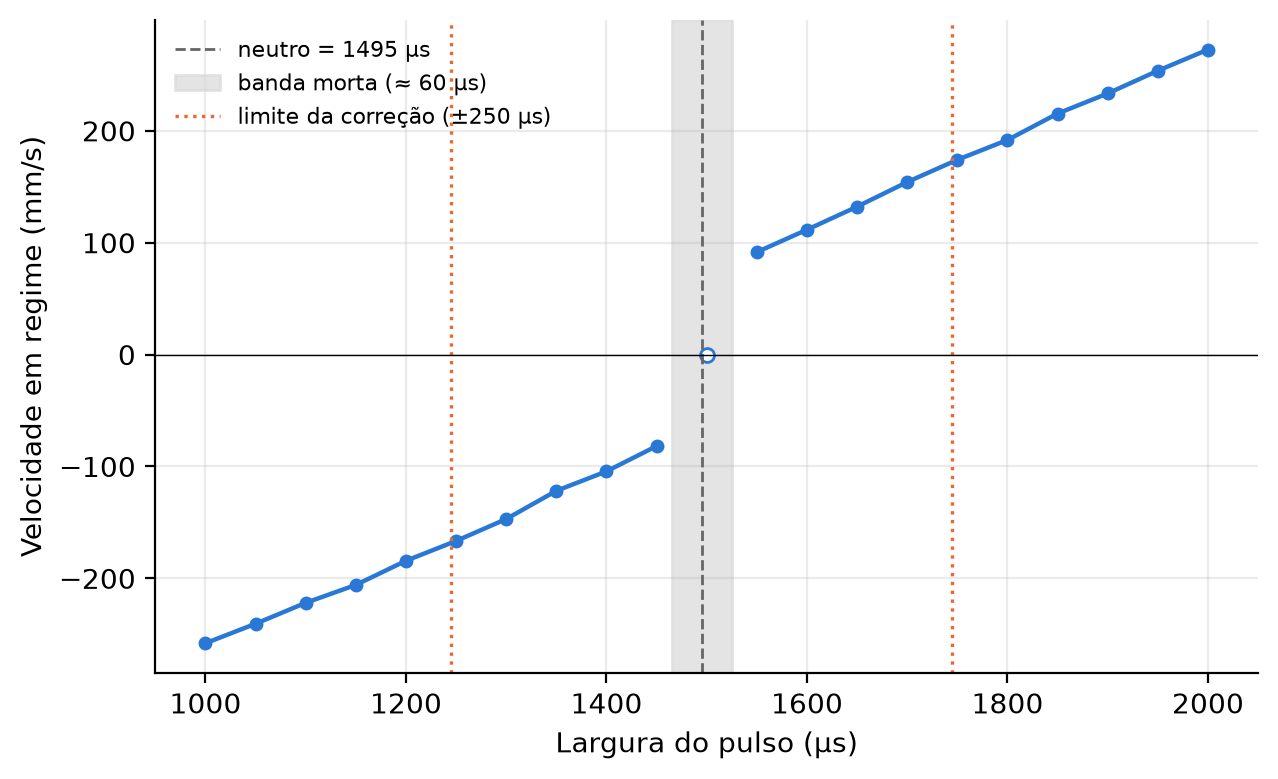
\includegraphics[width=0.78\linewidth]{curva_aberta.png}
  \caption{Pulso contra velocidade em regime, em malha aberta. A linha tracejada marca o neutro ($1495\unid{\mu s}$), a faixa cinza a banda morta ($\approx 60\unid{\mu s}$) e as linhas pontilhadas laranja os limites da correção do PID ($\pm 250\unid{\mu s}$).}
  \label{fig:curva}
\end{figure}

\paragraph{Banda morta.} A $1500\unid{\mu s}$ a roda não anda, e em $1450$ e $1550\unid{\mu s}$ já anda a $-81{,}8$ e $+91{,}6\unid{mm/s}$. A saída da banda é abrupta: a roda pula de $0$ para $\approx \pm 75$ a $80\unid{mm/s}$, sem passar por velocidades intermediárias. Com pulso fixo não existe velocidade sustentável entre $0$ e $\approx 75\unid{mm/s}$, o que limita o primeiro patamar da malha fechada.

\paragraph{Saturação.} Não há saturação clara dentro de 1000 a $2000\unid{\mu s}$. A curva segue quase linear até as pontas, com inclinação de $\approx 0{,}4\unid{mm/s}$ por $\mu$s ($0{,}38$ a $0{,}40$ do lado positivo e um pouco menos, $\approx 0{,}35$, perto de $1000\unid{\mu s}$). O limite que vale na malha fechada vem de outro lugar: a correção do PID é limitada a $\pm 250\unid{\mu s}$ em torno do neutro, ou seja, o pulso não passa de $1745\unid{\mu s}$, onde a curva dá $\approx 170\unid{mm/s}$.

\paragraph{Assimetria.} Os extremos são $+272{,}6$ e $-258{,}0\unid{mm/s}$, uma diferença de $14{,}6\unid{mm/s}$ ($5{,}4\,\%$). Na busca de 1300 a $1700\unid{\mu s}$, a $100\unid{\mu s}$ do neutro deram $+108{,}6$ e $-100{,}9\unid{mm/s}$ (cerca de $7\,\%$).

\paragraph{Repetibilidade.} Entre duas corridas da busca, a velocidade para um mesmo pulso variou em média $-6{,}5\unid{mm/s}$ do lado negativo e $+2{,}3\unid{mm/s}$ do positivo, com diferença máxima de $8{,}8\unid{mm/s}$ ($\approx 8\,\%$). Um pulso fixo não garante, então, uma velocidade fixa, e esse é o motivo de fechar a malha.

\section{Velocidade filtrada}
\label{sec:filtros}

A velocidade $\Delta s/\Delta t$ bruta tem passo de $9{,}5\unid{mm/s}$ e picos de ruído. Dois filtros foram comparados no mesmo registro de um degrau em malha aberta: pulso de $1700\unid{\mu s}$ a partir do repouso (regime em $152{,}4\unid{mm/s}$, medido com $t \ge 5\unid{s}$). Os parâmetros são:
\begin{itemize}[nosep]
  \item \textbf{média móvel} de $n$ amostras: $y[k] = \frac{1}{n}\sum_{j=0}^{n-1} v[k-j]$, com $n = 5$ (janela de $250\unid{ms}$);
  \item \textbf{passa-baixa de primeira ordem}: $y[k] = y[k-1] + \alpha\,(v[k] - y[k-1])$, com $\alpha = 0{,}3$.
\end{itemize}
A Figura~\ref{fig:filtros} mostra as duas saídas junto com a velocidade bruta, e a Tabela~\ref{tab:filtros} traz as métricas, incluindo outros parâmetros para ver a troca entre ruído e atraso.

\begin{figure}[htbp]
  \centering
  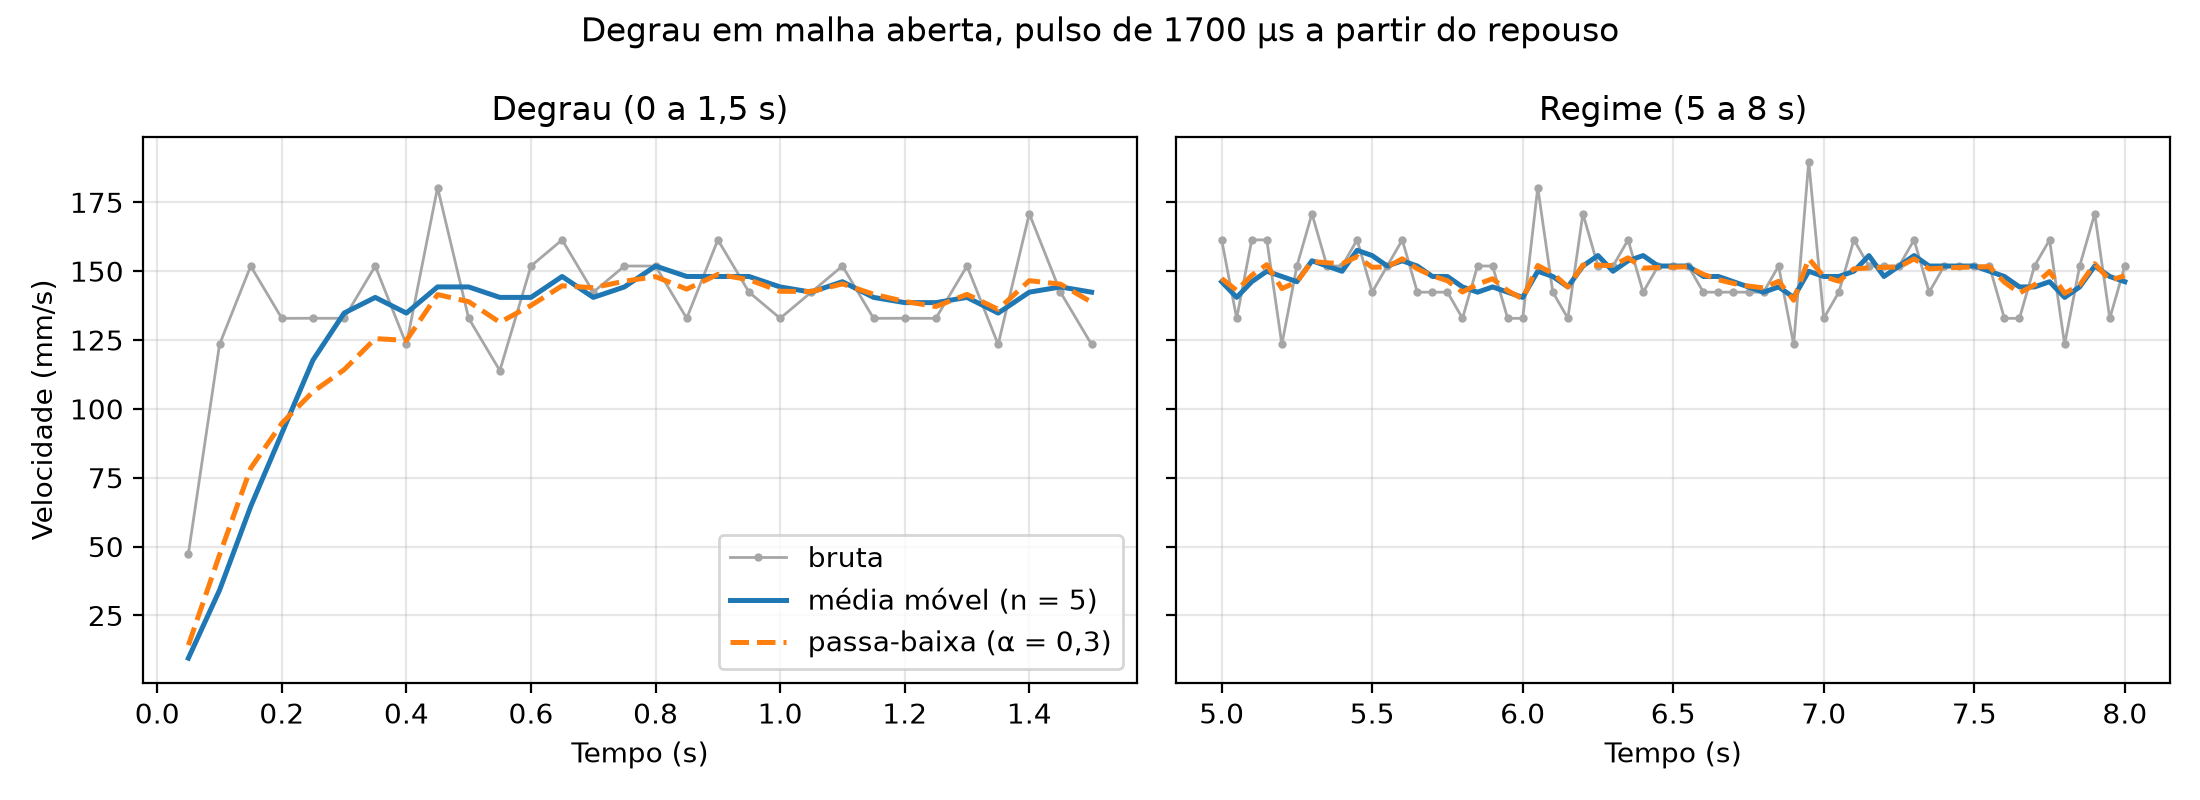
\includegraphics[width=\linewidth]{filtros_degrau.png}
  \caption{Degrau em malha aberta ($1700\unid{\mu s}$ a partir do repouso). À esquerda, o degrau; à direita, o regime. Velocidade bruta (cinza), média móvel com $n = 5$ (azul) e passa-baixa com $\alpha = 0{,}3$ (laranja).}
  \label{fig:filtros}
\end{figure}

\begin{table}[htbp]
\centering
\caption{Métricas dos filtros no degrau. O ruído é o desvio padrão em regime e o ruído de $dv/dt$ é o desvio padrão da derivada discreta. $t_{63}$ e $t_{90}$ são os tempos para chegar a $63{,}2\,\%$ e a $90\,\%$ do regime. Em negrito, os dois filtros comparados na Figura~\ref{fig:filtros}.}
\label{tab:filtros}
\small\setlength{\tabcolsep}{4pt}
\begin{tabular}{llrrrrr}
\toprule
Filtro & Parâm. & Desvio & Desvio $dv/dt$ & $t_{63}$ & $t_{90}$ & Pico \\
 & & (mm/s) & (mm/s$^2$) & (s) & (s) & (mm/s) \\
\midrule
Bruta       &                 & 13,16 & 429,4 & 0,082 & 0,124 & 189,8 \\
Média móvel & $n = 3$         & 5,38  & 105,8 & 0,139 & 0,217 & 155,1 \\
Média móvel & $\mathbf{n = 5}$& \textbf{4,49}  & \textbf{80,9}  & \textbf{0,210} & \textbf{0,321} & \textbf{155,7} \\
Média móvel & $n = 8$         & 3,44  & 50,2  & 0,316 & 0,438 & 154,2 \\
Média móvel & $n = 10$        & 2,85  & 39,8  & 0,386 & 0,546 & 152,8 \\
Passa-baixa & $\alpha = 0{,}15$ & 2,49 & 42,0 & 0,408 & 0,892 & 151,5 \\
Passa-baixa & $\mathbf{\alpha = 0{,}3}$ & \textbf{4,18} & \textbf{89,5} & \textbf{0,207} & \textbf{0,437} & \textbf{153,8} \\
Passa-baixa & $\alpha = 0{,}5$ & 6,28 & 163,5 & 0,129 & 0,331 & 162,4 \\
\bottomrule
\end{tabular}
\end{table}

\paragraph{Ruído.} Os dois filtros cortam o desvio em regime de $13{,}2$ para $\approx 4{,}3\unid{mm/s}$ (cerca de três vezes) e o ruído de $dv/dt$ de $429$ para $81$ a $90\unid{mm/s^2}$. A velocidade bruta tem picos de $190\unid{mm/s}$ num regime de $152\unid{mm/s}$.

\paragraph{Atraso.} Os dois levam $\approx 0{,}21\unid{s}$ para chegar a $63\,\%$, contra $0{,}08\unid{s}$ da bruta. A média móvel assenta em $0{,}32\unid{s}$ ($t_{90}$) e o passa-baixa em $0{,}44\unid{s}$, porque a resposta ao degrau do passa-baixa tem uma cauda longa. O atraso esperado da janela, $(n-1)/2 \cdot \Delta t = 0{,}1\unid{s}$, somado ao $t_{63}$ da bruta, dá $\approx 0{,}18\unid{s}$, perto dos $0{,}21\unid{s}$ medidos.

\paragraph{Escolha: média móvel com $n = 5$.} A malha final usa a média móvel de 5 amostras. As razões são:
\begin{enumerate}[nosep]
  \item o ruído em regime é o mesmo do passa-baixa ($4{,}5$ contra $4{,}2\unid{mm/s}$);
  \item o atraso inicial é o mesmo ($t_{63} = 0{,}21\unid{s}$), mas a média móvel assenta mais cedo ($0{,}32$ contra $0{,}44\unid{s}$), e o atraso do filtro entra na malha fechada: quanto maior, menores os ganhos que ela aguenta;
  \item o ruído em $dv/dt$ é um pouco menor ($81$ contra $90\unid{mm/s^2}$), o que importa para o termo derivativo, que age na velocidade filtrada;
  \item o pico do degrau fica $2\,\%$ acima do regime, dentro do ruído, então o filtro não cria sobressinal próprio;
  \item $n = 8$ e $n = 10$ cortam mais o ruído ($3{,}4$ e $2{,}8\unid{mm/s}$), mas o $t_{90}$ vai a $0{,}44$ e $0{,}55\unid{s}$, e $\alpha = 0{,}15$ leva $0{,}89\unid{s}$ para chegar a $90\,\%$, alto demais para patamares de $3\unid{s}$; $n = 3$ ainda deixa $5{,}4\unid{mm/s}$ de ruído, e $\alpha = 0{,}5$ passa $6{,}6\,\%$ do regime no pico.
\end{enumerate}
A escolha vem de uma resposta em malha aberta, e a malha fechada é que decide de verdade. Os ensaios foram feitos todos com a média móvel, e o passa-baixa não foi testado em malha fechada.

\section{Controle PID}

\subsection{Lei de controle e limites}

O erro é $e = v_{\mathrm{ped}} - v_{\mathrm{filt}}$, com a velocidade pedida e a filtrada em mm/s. A saída do PID é uma correção em microssegundos, somada ao neutro:
\begin{equation}
  u = k_p\,e + k_i \int e\,dt - k_d\,\frac{dv_{\mathrm{filt}}}{dt}, \qquad
  \text{pulso} = 1495 + u\ (\mu\text{s}).
\end{equation}
O termo derivativo, quando usado, age sobre a velocidade medida já filtrada, e não sobre o erro. O $\Delta t$ da integral e da derivada é o intervalo medido entre as leituras ($\approx 50\unid{ms}$). Os limites são:
\begin{itemize}[nosep]
  \item a integral é limitada de modo que $k_i \int e\,dt$ não passe de $\pm 250\unid{\mu s}$, e é \textbf{zerada} sempre que o setpoint muda, para não carregar o erro antigo;
  \item a correção $u$ é limitada a $\pm 250\unid{\mu s}$ em torno do neutro;
  \item o pulso resultante fica entre $1000$ e $2000\unid{\mu s}$ (com a correção limitada, na prática entre $1245$ e $1745\unid{\mu s}$).
\end{itemize}
As unidades dos ganhos são $k_p$ em $\mu$s/(mm/s), $k_i$ em $\mu$s/(mm/s)/s e $k_d$ em $\mu$s/(mm/s$^2$).

\subsection{Sintonia}

A sintonia seguiu o procedimento do enunciado, um ganho por vez, olhando um degrau de $0$ a $150\unid{mm/s}$ por $4\unid{s}$ a partir do repouso. Com $k_i = k_d = 0$, subiu-se $k_p$ até a resposta oscilar. Depois subiu-se $k_i$ até o erro de regime sumir. O $k_d$ não foi usado, porque o sobressinal ficou pequeno e o ruído de $dv/dt$ ($81\unid{mm/s^2}$ mesmo filtrado) iria direto para o pulso. A Tabela~\ref{tab:pid} resume as tentativas, e a Figura~\ref{fig:pid} mostra os cinco degraus. Nos valores de regime, a velocidade é a média dos últimos instantes do degrau (a partir de $2{,}5\unid{s}$ para T01 a T03, e dos últimos $1{,}5\unid{s}$ para T04 e T05).

\begin{table}[htbp]
\centering
\caption{Tentativas de sintonia (setpoint de $150\unid{mm/s}$, média móvel $n = 5$, neutro $1495\unid{\mu s}$). $k_p$ em $\mu$s/(mm/s) e $k_i$ em $\mu$s/(mm/s)/s.}
\label{tab:pid}
\begin{tabularx}{\linewidth}{lrrrrL}
\toprule
Tent. & $k_p$ & $k_i$ & $v$ regime (mm/s) & Erro (mm/s) & O que o gráfico fez $\rightarrow$ decisão \\
\midrule
T01 & 1 & 0 & 87,6 & 62,4 (42\,\%) & Sem oscilação, sobe em $0{,}25\unid{s}$. Pulso em $1557{,}6 \pm 2{,}5\unid{\mu s}$. $\rightarrow$ subir $k_p$. \\
T02 & 3 & 0 & 110,3 & 39,7 (26\,\%) & Sem oscilação. Primeiro pulso satura em $1745\unid{\mu s}$ e o pico passa do valor final. $\rightarrow$ subir $k_p$. \\
T03 & 6 & 0 & 123,9 & 26,1 (17\,\%) & Começa a oscilar: pulso de $1598$ a $1700\unid{\mu s}$ (desvio $27{,}7\unid{\mu s}$), período $\approx 0{,}35\unid{s}$. $\rightarrow$ $K_u \approx 6$, voltar a $k_p = 3$ e subir $k_i$. \\
T04 & 3 & 3 & 145,1 & 4,9 (3\,\%) & Sem oscilação, sem sobressinal, mas lento: ainda sobe aos $4\unid{s}$. $\rightarrow$ subir $k_i$. \\
T05 & 3 & 8 & 150,0 & 0,0 & Erro zero, $t_{63} = 0{,}25\unid{s}$ e $t_{90} = 0{,}35\unid{s}$. Sobressinal de $7{,}6\,\%$ (pico $161{,}3\unid{mm/s}$) com o pulso saturado no início. $\rightarrow$ adotar. \\
\bottomrule
\end{tabularx}
\end{table}

\begin{figure}[htbp]
  \centering
  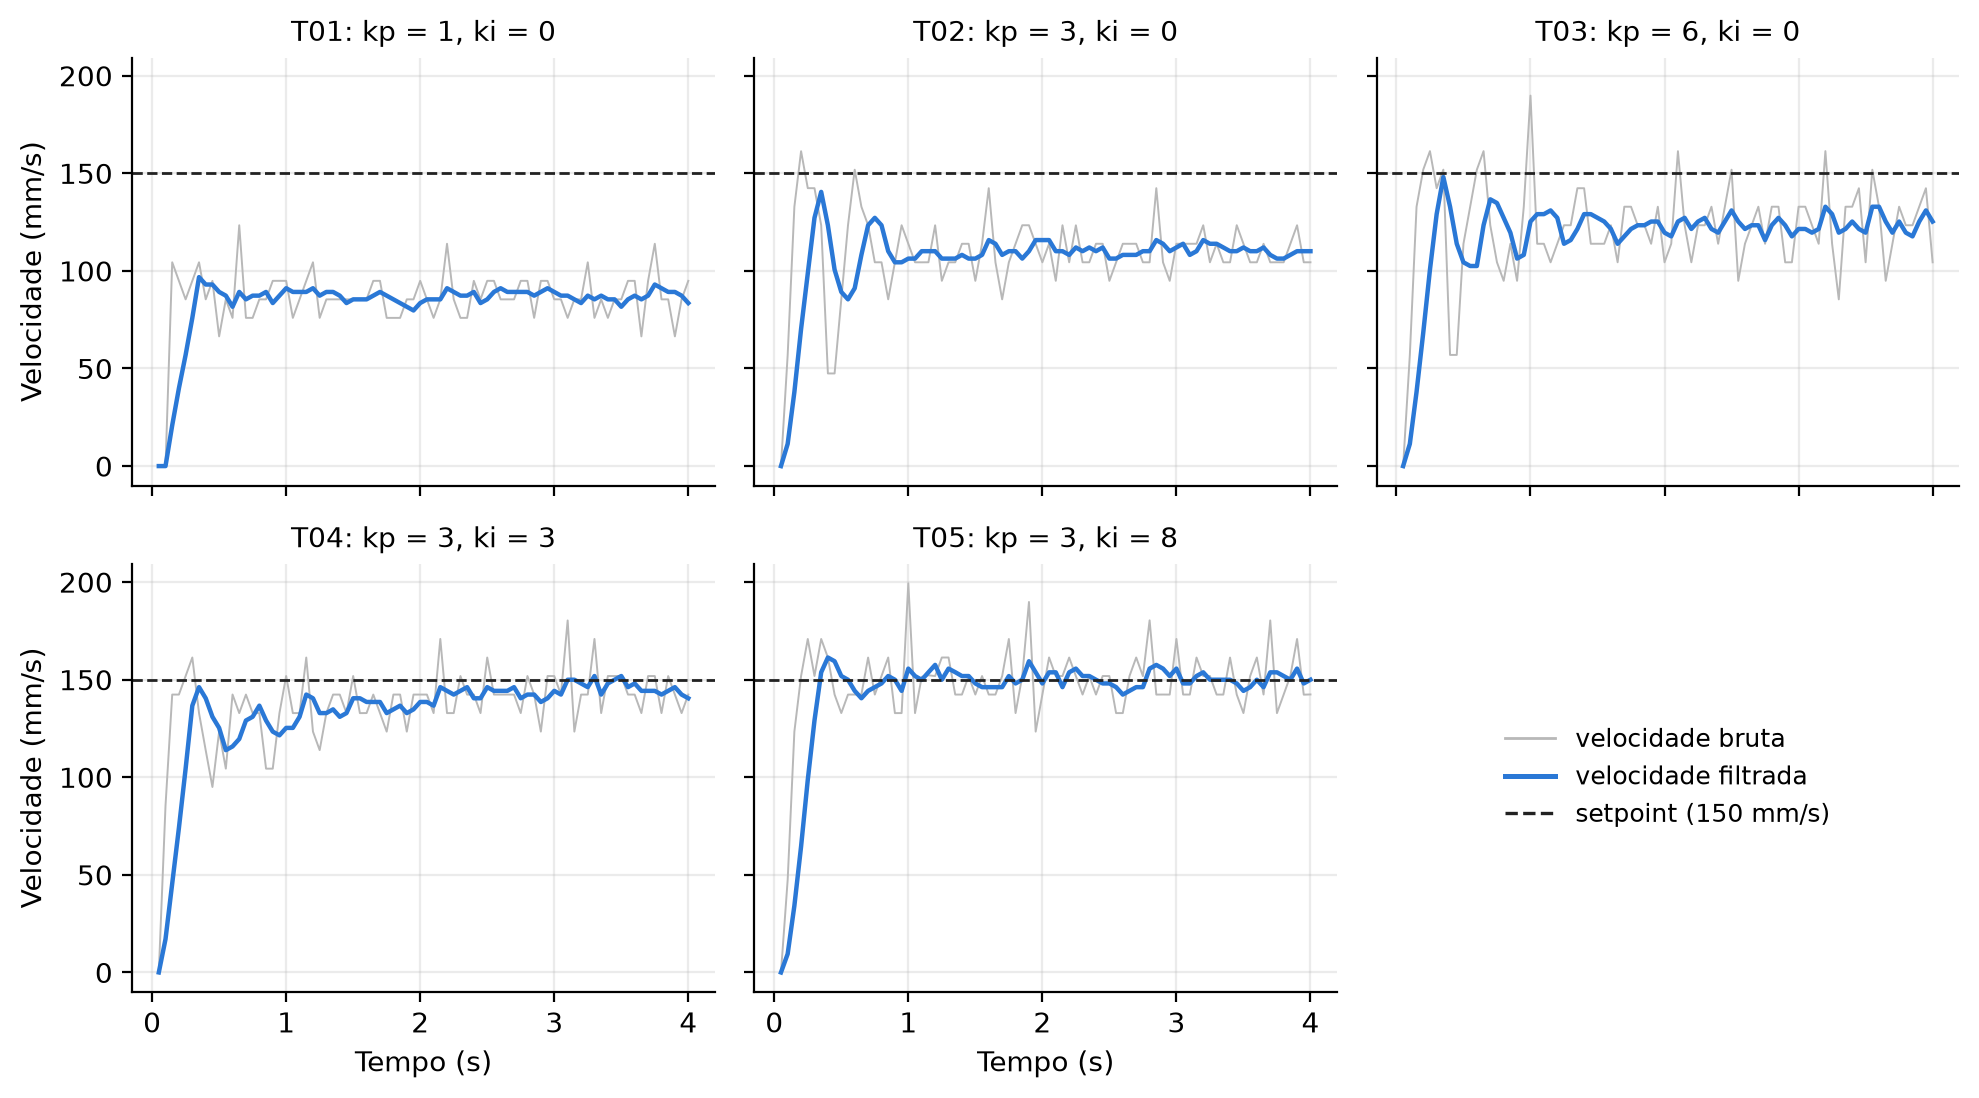
\includegraphics[width=\linewidth]{pid_sintonia.png}
  \caption{Degraus de $0$ a $150\unid{mm/s}$ nas cinco tentativas de sintonia. Velocidade bruta (cinza), filtrada (azul) e setpoint (tracejado).}
  \label{fig:pid}
\end{figure}

\paragraph{O erro com só $k_p$.} Com só o termo proporcional a correção $u = k_p e$ exige um erro de regime para existir. Para $150\unid{mm/s}$ a curva aberta pede $\approx 1660\unid{\mu s}$ (correção de $\approx +165\unid{\mu s}$), mas com $k_p = 1$ a malha se acomoda em $1557\unid{\mu s}$, onde a curva dá $\approx 90\unid{mm/s}$. Com o ganho da planta de $\approx 0{,}4\unid{mm/s}$ por $\mu$s acima da banda morta, o erro de regime de um controle só P fica em torno de $84/(1 + 0{,}4\,k_p)\unid{mm/s}$, o que dá $\approx 60$, $38$ e $25\unid{mm/s}$ para $k_p = 1$, $3$ e $6$. Os erros medidos foram $62{,}4$, $39{,}7$ e $26{,}1\unid{mm/s}$, e o modelo bate. Só o termo integral zera esse erro.

\paragraph{Ganhos finais.} Os ganhos finais são
\begin{equation}
  k_p = 3\ \mu\text{s/(mm/s)}, \qquad k_i = 8\ \mu\text{s/(mm/s)/s}, \qquad k_d = 0,
\end{equation}
com a média móvel de $n = 5$. Da T03 saíram $K_u \approx 6$ e $T_u \approx 0{,}35\unid{s}$; o Ziegler--Nichols daria $k_p = 0{,}6 K_u \approx 3{,}6$ e $k_i = 1{,}2 K_u/T_u \approx 21$. O $k_p$ de $3$ ficou perto disso, mas o $k_i$ de $21$ é agressivo para esta planta, e $k_i = 8$ já zerou o erro. Uma tentativa intermediária com $k_i = 5$, para ver se o sobressinal cairia, não foi feita, e os ensaios usaram os ganhos da T05.

\section{Resultados}

Os três ensaios usam a mesma malha, os mesmos ganhos e o mesmo filtro. Condição declarada: neutro $1495\unid{\mu s}$; $k = 0{,}4746\unid{mm/tick}$; $\Delta t = 50\unid{ms}$; $k_p = 3$, $k_i = 8$, $k_d = 0$; média móvel de $n = 5$; correção limitada a $\pm 250\unid{\mu s}$; MG90S novo. Em cada gráfico, o eixo horizontal é o tempo em segundos a partir do repouso, e o pulso comandado vai num painel abaixo, com o neutro e os limites de $\pm 250\unid{\mu s}$.

\subsection{Ensaio 1: cinco patamares}

A roda parte do repouso e percorre cinco velocidades positivas em ordem crescente, $100$, $115$, $130$, $145$ e $160\unid{mm/s}$, $3\unid{s}$ cada (Figura~\ref{fig:e1}). Foram escolhidas dentro do que a malha segura: acima de $\approx 80\unid{mm/s}$ (saída da banda morta) e até $\approx 165\unid{mm/s}$ (Seção~\ref{sec:disc}). Os valores da Tabela~\ref{tab:e1} são do último $1\unid{s}$ de cada patamar.

\begin{figure}[htbp]
  \centering
  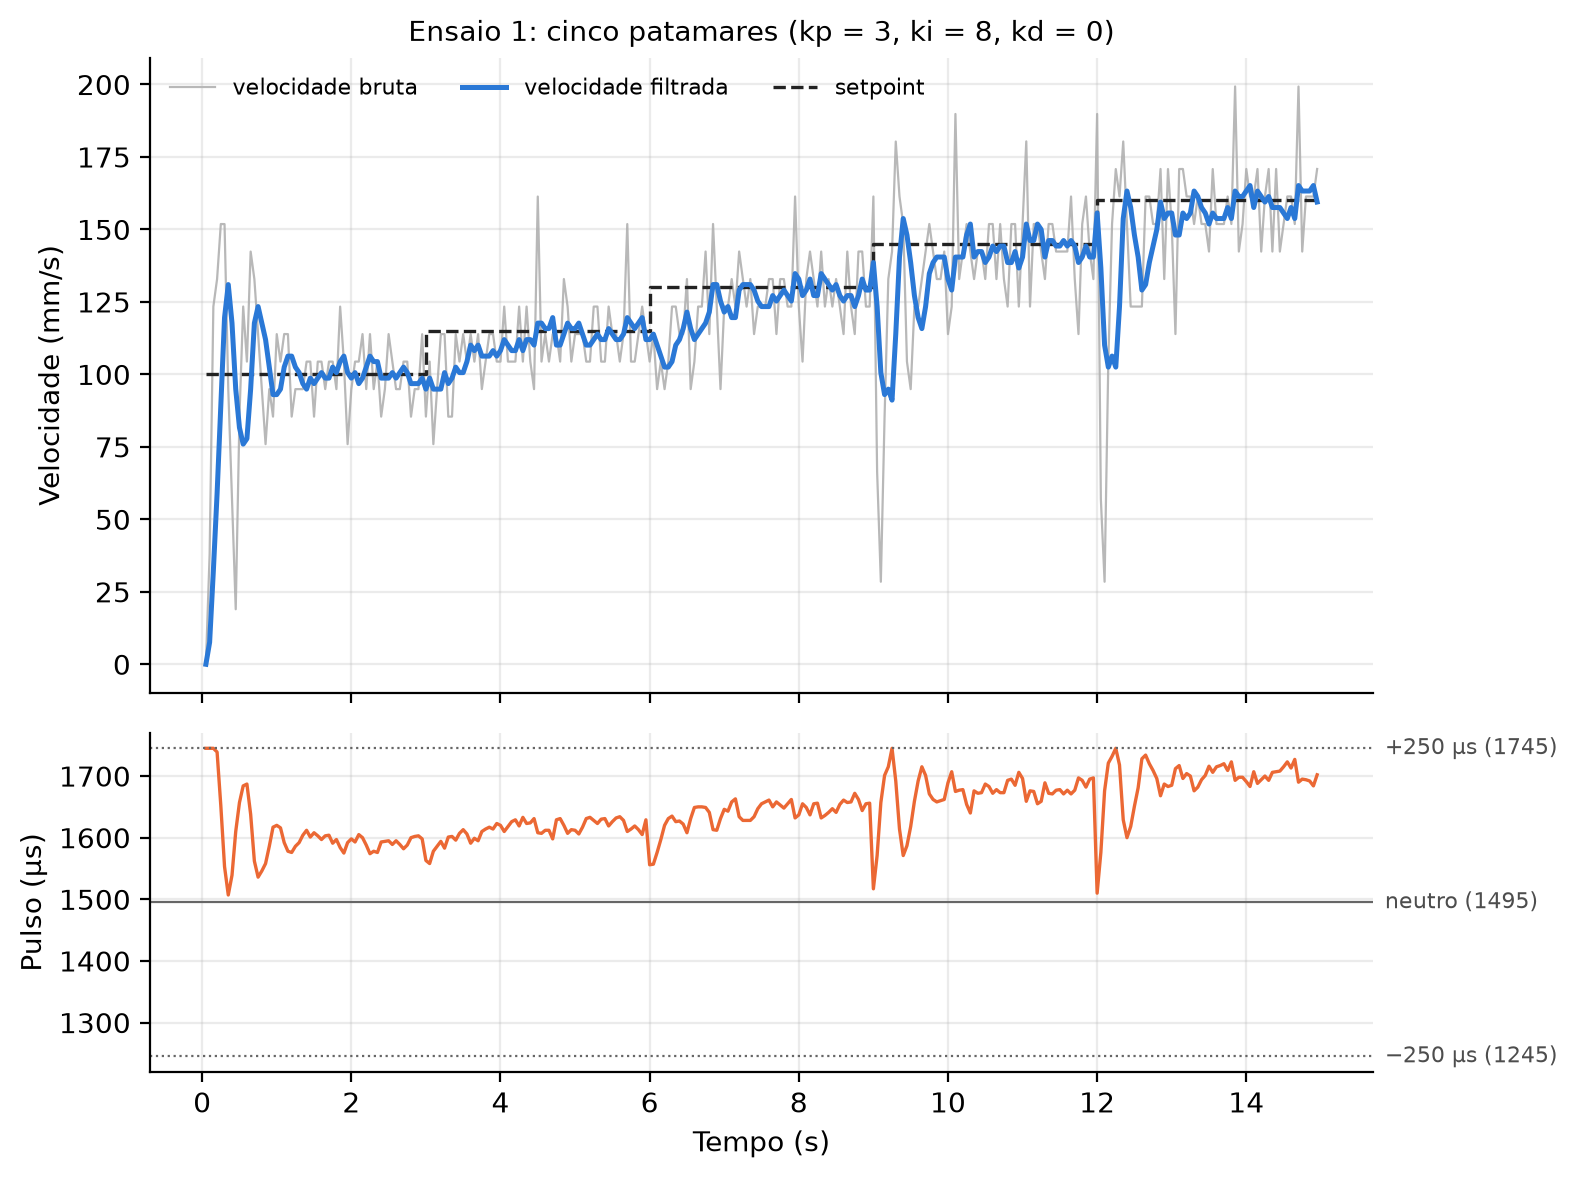
\includegraphics[width=0.92\linewidth]{ensaio1_patamares.png}
  \caption{Ensaio 1: cinco patamares. Setpoint (tracejado), velocidade filtrada (azul) e bruta (cinza), e o pulso no painel de baixo.}
  \label{fig:e1}
\end{figure}

\begin{table}[htbp]
\centering
\caption{Ensaio 1. Regime no último $1\unid{s}$ de cada patamar.}
\label{tab:e1}
\small\setlength{\tabcolsep}{4pt}
\begin{tabular}{rrrrrr}
\toprule
Patamar & $v$ média & Erro & Desvio de $v$ & Sobre- & Pulso médio \\
(mm/s) & (mm/s) & (mm/s) & (mm/s) & sinal & ($\mu$s) \\
\midrule
100 & 100,0 & 0,0 (0,0\,\%) & 2,7 & 31,0\,\% & 1592 \\
115 & 114,4 & 0,6 (0,5\,\%) & 2,9 & 4,0\,\%  & 1622 \\
130 & 129,2 & 0,8 (0,6\,\%) & 2,9 & 3,7\,\%  & 1650 \\
145 & 144,7 & 0,3 (0,2\,\%) & 3,7 & 6,0\,\%  & 1678 \\
160 & 160,2 & $-0{,}2$ ($-0{,}1\,\%$) & 3,6 & 3,2\,\% & 1701 \\
\bottomrule
\end{tabular}
\end{table}

\paragraph{Tempo de subida do primeiro degrau.} De $0$ a $100\unid{mm/s}$, a velocidade filtrada chega a $63\,\%$ em $0{,}25\unid{s}$ e a $90\,\%$ em $0{,}30\unid{s}$. O sobressinal é de $31\,\%$ (pico de $131\unid{mm/s}$), porque o pulso satura em $1745\unid{\mu s}$ no início e o integrador acumula enquanto a velocidade sobe.

\paragraph{Erro nos patamares.} O erro de regime é de no máximo $0{,}6\,\%$ em todos os patamares, e o pulso médio de cada um acompanha a curva aberta ($1592\unid{\mu s}$ para $100\unid{mm/s}$ e $1701\unid{\mu s}$ para $160\unid{mm/s}$).

\paragraph{A integral na troca de patamar.} A integral é zerada em cada troca, então não há erro antigo carregado: o sobressinal cai de $31\,\%$ no primeiro degrau para $3$ a $6\,\%$ nos seguintes, e o erro volta a ficar abaixo de $1\,\%$ antes do fim dos $3\unid{s}$. O custo é que a integral recomeça do zero em cada degrau, e para degraus pequenos ($15\unid{mm/s}$) o tempo de assentamento fica entre $0$ e $1{,}5\unid{s}$ e é dominado pelo ruído de $\approx 3\unid{mm/s}$ da velocidade filtrada, então não é uma medida confiável.

\subsection{Ensaio 2: inversão de sentido}

A roda anda a $+120\unid{mm/s}$ por $4\unid{s}$ e em seguida a $-120\unid{mm/s}$ por mais $4\unid{s}$, passando pelo zero (Figura~\ref{fig:e2}).

\begin{figure}[htbp]
  \centering
  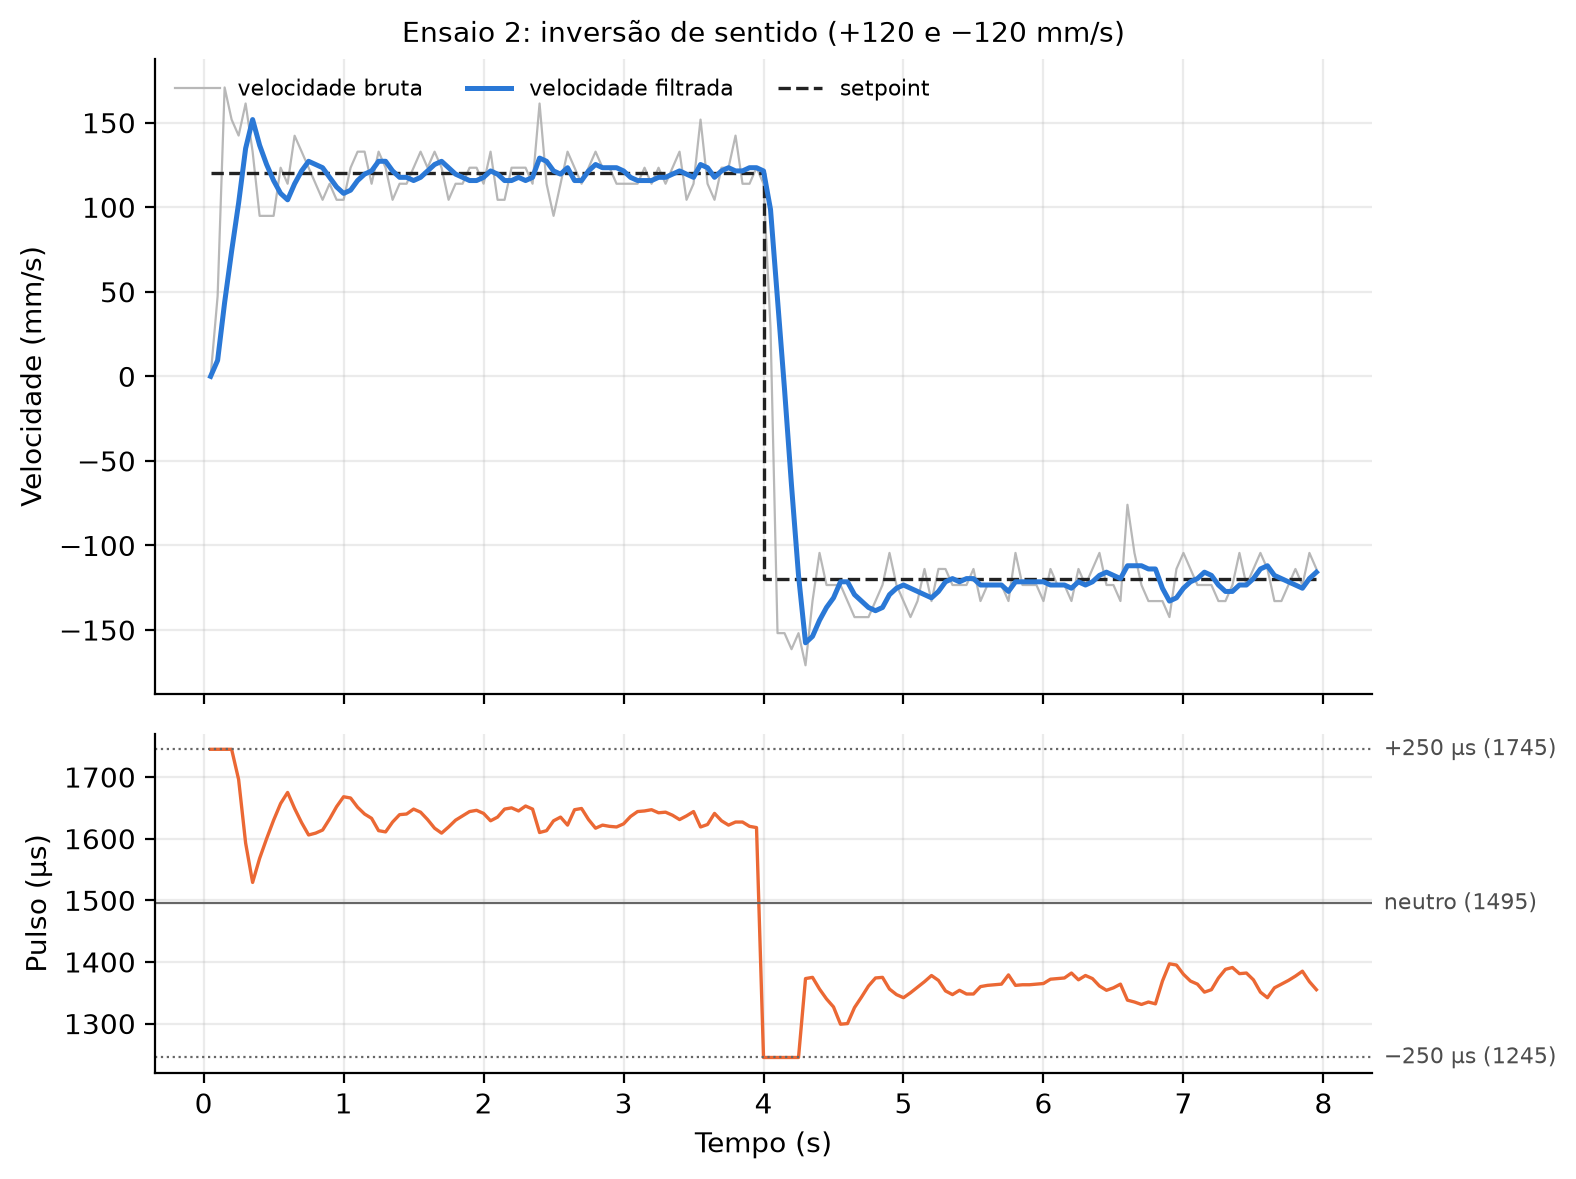
\includegraphics[width=0.92\linewidth]{ensaio2_inversao.png}
  \caption{Ensaio 2: inversão de sentido, de $+120$ a $-120\unid{mm/s}$ em $t = 4\unid{s}$.}
  \label{fig:e2}
\end{figure}

\begin{itemize}[nosep]
  \item \textbf{Regime:} $120{,}1\unid{mm/s}$ no sentido positivo (pulso de $1633\unid{\mu s}$) e $-120{,}6\unid{mm/s}$ no negativo ($1369\unid{\mu s}$), com erros de $0{,}1$ e $0{,}5\unid{mm/s}$.
  \item \textbf{Banda morta na passagem:} na troca, o pulso vai direto para $1245\unid{\mu s}$ (saturado em $-250\unid{\mu s}$, bem abaixo da banda morta) por $0{,}25\unid{s}$. A roda passa por zero $0{,}15\unid{s}$ depois da troca, atravessando a banda morta sem parar nela, e chega a $-117{,}7\unid{mm/s}$ em $0{,}25\unid{s}$.
  \item \textbf{Tempo até o setpoint novo:} há sobressinal de $31\,\%$ para o lado negativo (pico de $-157{,}6\unid{mm/s}$ em $0{,}3\unid{s}$ depois da troca), por causa da saturação e do integrador zerado, e a velocidade assenta em $-121{,}5\unid{mm/s}$ em $\approx 0{,}55\unid{s}$.
  \item \textbf{Sentido do encoder:} os ticks descem de $+1001$ para $-20$ quando a velocidade fica negativa, então o sinal do encoder concorda com o da velocidade, e não foi preciso trocar A e B.
  \item O deslocamento líquido é de $-9{,}5\unid{mm}$ ($-20$ ticks), depois de $\approx 475\unid{mm}$ para cada lado.
\end{itemize}

\subsection{Ensaio 3: distância}

O ensaio andou três voltas da roda a $120\unid{mm/s}$ e cortou o pulso no neutro ao atingir $3\pi D = 409{,}04\unid{mm}$ (Figura~\ref{fig:e3}). A velocidade média antes do corte foi de $120{,}6\unid{mm/s}$. A roda chegou a $410{,}5\unid{mm}$ em $3{,}45\unid{s}$, quando o pulso foi cortado; depois, ainda andou $3{,}8\unid{mm}$ e \textbf{parou em $s = 414{,}78\unid{mm}$} (874 ticks), em cerca de $0{,}3\unid{s}$. O valor esperado de $3\pi D$ dá 862 ticks, então a diferença é de $+5{,}7\unid{mm}$ ($+1{,}4\,\%$). A conferência à mão, contando as três voltas da roda, deu ``praticamente exatas'', o que concorda com essa diferença pequena.

\begin{figure}[htbp]
  \centering
  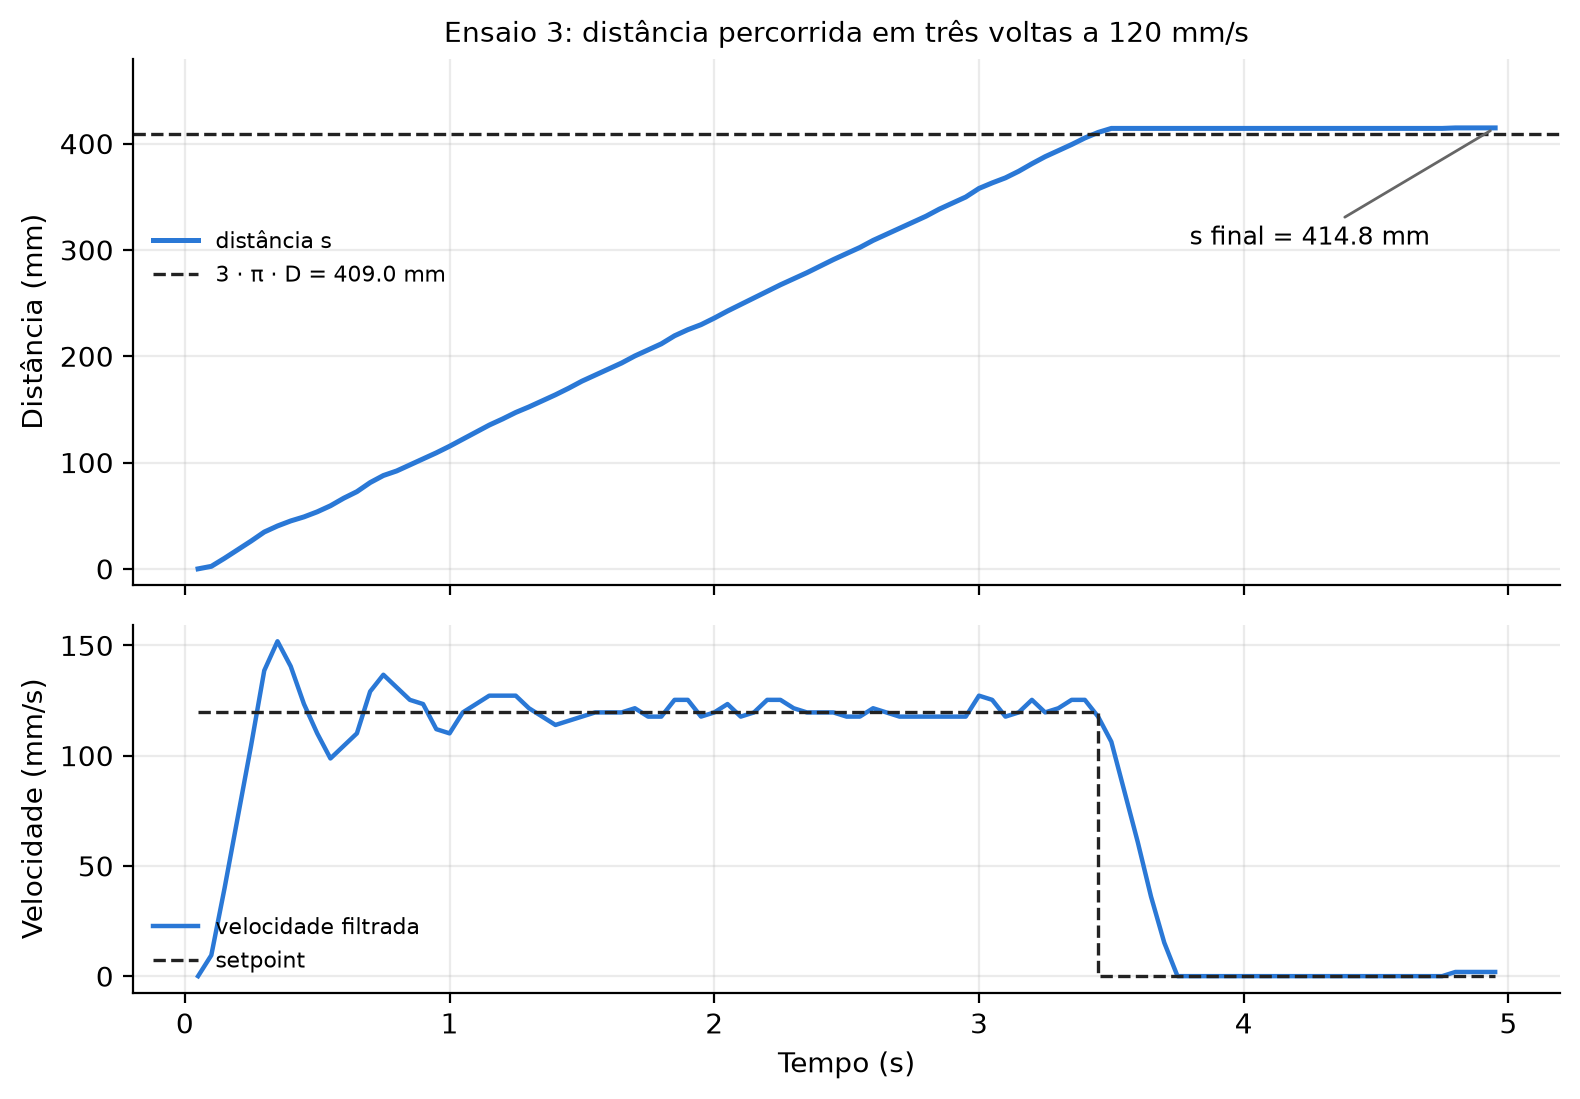
\includegraphics[width=0.92\linewidth]{ensaio3_distancia.png}
  \caption{Ensaio 3: distância $s(t)$ em três voltas a $120\unid{mm/s}$ (em cima), com o valor de $3\pi D = 409{,}0\unid{mm}$, e a velocidade (embaixo).}
  \label{fig:e3}
\end{figure}

Os $5{,}7\unid{mm}$ de diferença vêm de duas causas: o alvo é testado a cada amostra de $50\unid{ms}$ e, a $120\unid{mm/s}$, a roda anda $\approx 6\unid{mm}$ por amostra, então o corte pode ocorrer até $6\unid{mm}$ depois do alvo; e depois do corte a roda ainda desliza $3{,}8\unid{mm}$. A incerteza de $k$ e de $N$ pesa menos ($\approx 1\unid{mm}$ em $409\unid{mm}$).

\section{Discussão}
\label{sec:disc}

\paragraph{O que a curva aberta explica nos degraus.} O salto de $0$ a $\approx 80\unid{mm/s}$ na saída da banda morta (Figura~\ref{fig:curva}) explica o sobressinal de $31\,\%$ do primeiro patamar: para tirar a roda do repouso o pulso tem de atravessar $\approx 30\unid{\mu s}$ de banda morta, e a roda aparece de uma vez a $\approx 80\unid{mm/s}$; o PID, que viu um erro de $100\unid{mm/s}$ e saturou em $+250\unid{\mu s}$ até a velocidade subir, empurra a roda além do setpoint (pico de $131\unid{mm/s}$) antes de recuar. A mesma banda explica a inversão: o pulso cruza o neutro com a saturação em $-250\unid{\mu s}$ e a roda passa por zero em $0{,}15\unid{s}$, sem se deter. Ela também explica por que o patamar mais baixo ($100\unid{mm/s}$) já está perto do limite inferior da malha: abaixo de $\approx 80\unid{mm/s}$, um pulso fixo não segura nenhuma velocidade. A inclinação da curva ($\approx 0{,}4\unid{mm/s}$ por $\mu$s) é a que explica o modelo de erro do controle só P, e os pulsos médios de regime dos patamares (Tabela~\ref{tab:e1}) caem em cima da curva medida.

\paragraph{O que o filtro atrasou.} A média móvel de 5 amostras acrescenta $\approx 0{,}1\unid{s}$ de atraso à medida ($t_{63}$ de $0{,}21\unid{s}$ contra $0{,}08\unid{s}$ da bruta). Esse atraso limita o ganho: com $k_p = 6$ a malha já mostrava uma oscilação de período $\approx 0{,}35\unid{s}$, da ordem do atraso somado do filtro e do servo. Em troca, o ruído de $13$ para $4{,}5\unid{mm/s}$ foi o que deixou o pulso utilizável: sem filtro, um erro de quantização de $9{,}5\unid{mm/s}$ virava $\pm 28\unid{\mu s}$ de pulso com $k_p = 3$ a cada amostra. Por isso o $k_d$ ficou em zero: mesmo filtrado, $dv/dt$ tem ruído de $81\unid{mm/s^2}$, e ele iria direto para o servo.

\paragraph{Onde a malha saturou nos $\pm 250\,\mu$s.} Esta foi a principal limitação. O servo chega a $272\unid{mm/s}$ em malha aberta, mas a correção do enunciado só deixa o pulso ir a $1745\unid{\mu s}$, e a malha não passa de $\approx 165\unid{mm/s}$. Uma primeira corrida do ensaio 1, com patamares de $100$, $130$, $160$, $190$ e $220\unid{mm/s}$, mostrou isso (Figura~\ref{fig:e1sat}): os dois últimos ficaram em $167{,}0$ e $167{,}6\unid{mm/s}$, com erros de $23{,}0$ e $52{,}4\unid{mm/s}$ ($12$ e $24\,\%$) e o pulso colado em $1745\unid{\mu s}$. A faixa útil da malha, então, vai de $\approx 80$ a $\approx 165\unid{mm/s}$, e foi nela que o ensaio 1 foi refeito. A saturação também aparece no início de todo degrau grande, e é a causa dos sobressinais de $31\,\%$ (ensaios 1 e 2). Quem quiser mais velocidade tem de aumentar o limite da correção. A integral limitada ($\pm 250\unid{\mu s}$) e zerada na troca de setpoint não evita o acúmulo durante a saturação inicial; uma lógica de \textit{anti-windup} que pare de integrar quando o pulso está saturado poderia reduzir esse sobressinal, mas não foi testada.

\begin{figure}[htbp]
  \centering
  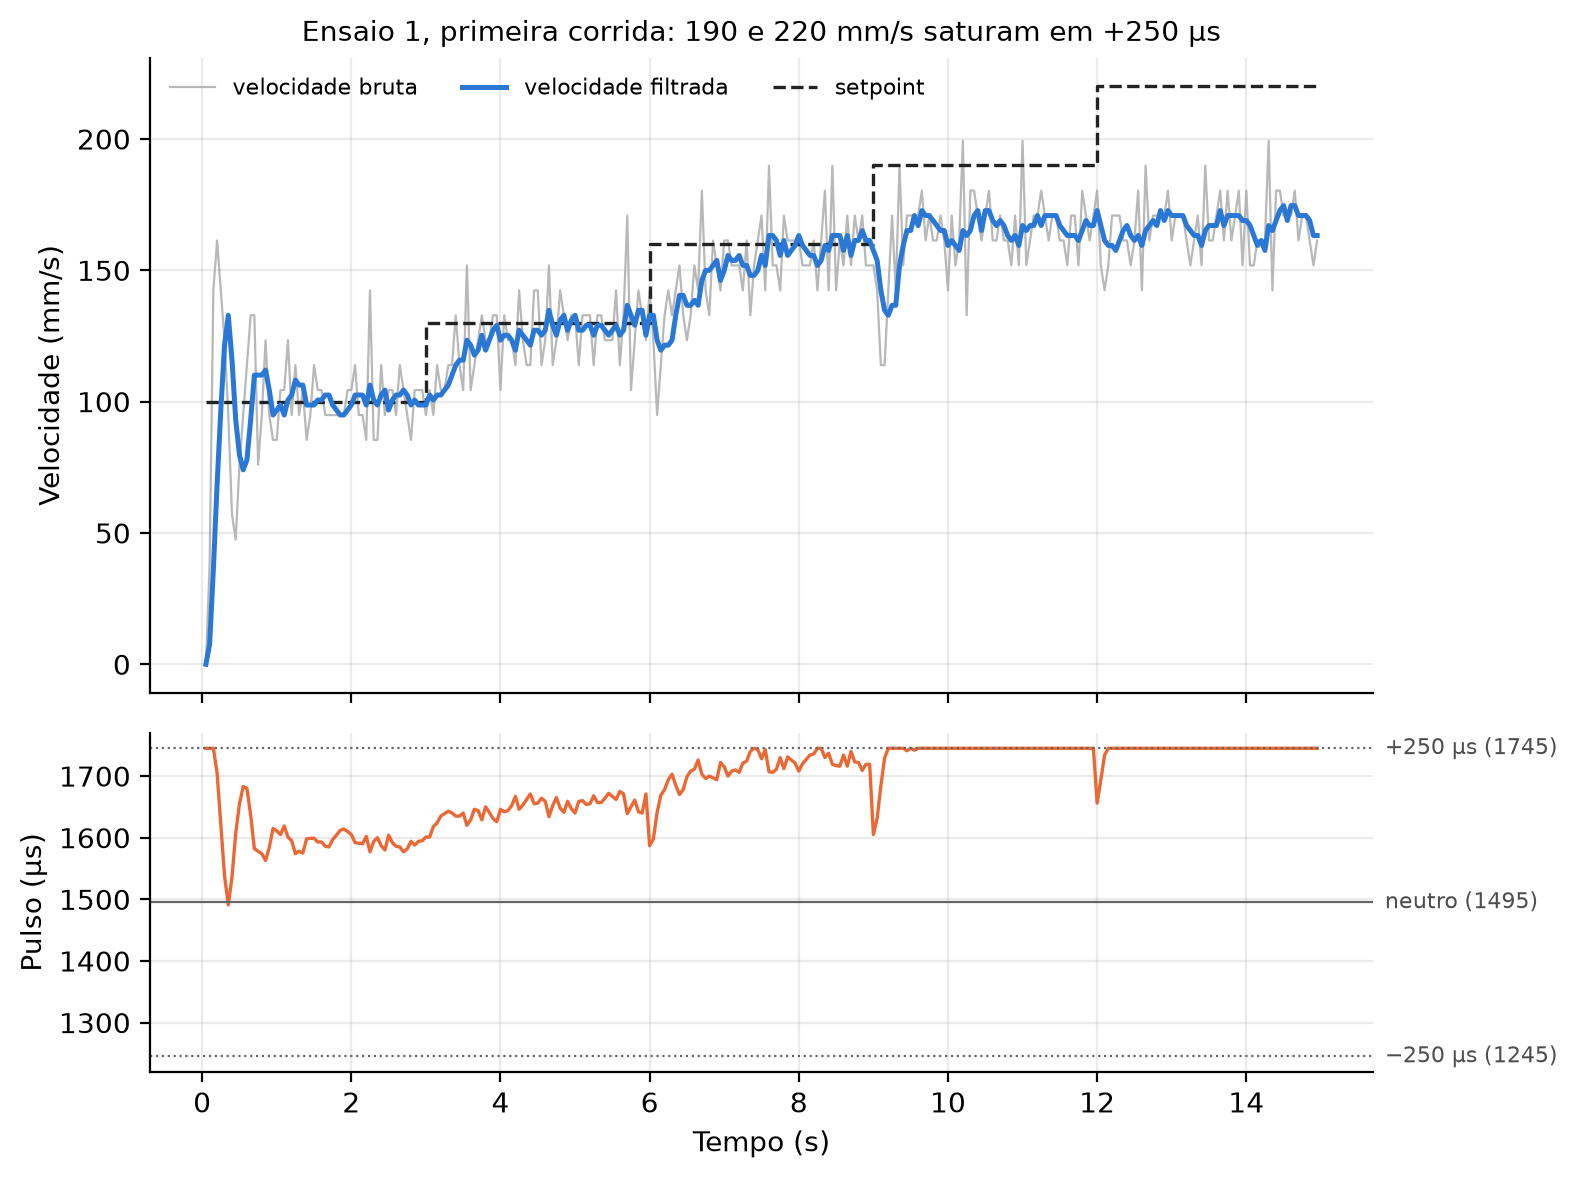
\includegraphics[width=0.92\linewidth]{ensaio1_saturado.png}
  \caption{Primeira corrida do ensaio 1, com patamares de $190$ e $220\unid{mm/s}$ fora do alcance da malha. O pulso fica em $1745\unid{\mu s}$ ($+250\unid{\mu s}$) e a velocidade para em $\approx 167\unid{mm/s}$.}
  \label{fig:e1sat}
\end{figure}

\paragraph{O que não ficou bom.}
\begin{itemize}[nosep]
  \item \textbf{Sobressinal de $31\,\%$} no primeiro degrau do ensaio 1 e no cruzamento do ensaio 2, resultado da saturação e do salto da banda morta.
  \item \textbf{Ruído na velocidade filtrada:} $\approx 3$ a $4\unid{mm/s}$ em regime ($\approx 2{,}5\,\%$ do setpoint), com o pulso oscilando $\pm 12\unid{\mu s}$. O degrau de $9{,}5\unid{mm/s}$ não permite menos sem aumentar o $\Delta t$ ou o atraso do filtro.
  \item \textbf{Repetibilidade do servo:} a velocidade para um mesmo pulso varia $\approx \pm 5\unid{mm/s}$ entre corridas (até $8{,}8\unid{mm/s}$), e o pulso médio para $160\unid{mm/s}$ foi de $1726\unid{\mu s}$ na primeira corrida do ensaio 1 e de $1701\unid{\mu s}$ na segunda. Cada ensaio foi feito uma única vez com a malha final, então não há estatística da repetibilidade da malha.
  \item \textbf{Sintonia incompleta:} a tentativa com $k_i = 5$ não foi feita, o $k_d$ nunca foi testado, e a comparação dos filtros não foi refeita em malha fechada.
  \item \textbf{Troca de motores:} três servos foram usados, e só os dados do MG90S novo valem. Uma busca do neutro anterior, com $1485\unid{\mu s}$, não foi reproduzida.
  \item \textbf{Ensaio 3:} a primeira corrida mandava o setpoint para $0$ ao atingir o alvo e mantinha a malha ativa. Por causa da banda morta, a malha não consegue segurar velocidades entre $-80$ e $+80\unid{mm/s}$ e ficou caçando o zero, com o pulso indo de $1245$ a $1745\unid{\mu s}$ e a distância oscilando entre $383$ e $412\unid{mm}$ por $1{,}5\unid{s}$. A correção foi cortar o pulso no neutro ao atingir o alvo, em malha aberta. Isso mostra que esta malha não serve para parar em posição, e que o erro de $5{,}7\unid{mm}$ poderia cair se o corte fosse antecipado em $\approx 4\unid{mm}$ (distância de frenagem a $120\unid{mm/s}$).
  \item \textbf{Alimentação:} \pendente{condição de alimentação do servo (USB, fonte externa ou pilhas) em cada ensaio}.
\end{itemize}

\section{Conclusão}

A roda monta-se com $D = 43{,}40\unid{mm}$ e $N = 287{,}3$ ticks por volta, o que dá $k = 0{,}4746\unid{mm/tick}$, e o encoder lido a $50\unid{ms}$ resolve a velocidade em degraus de $9{,}5\unid{mm/s}$. O servo tem neutro de $1495\unid{\mu s}$, banda morta de $\approx 60\unid{\mu s}$, um salto de $0$ a $\approx 80\unid{mm/s}$ na saída dela e uma curva quase linear até $\pm 270\unid{mm/s}$ em malha aberta. Com a velocidade filtrada por média móvel de 5 amostras e um PI de $k_p = 3\unid{\mu s/(mm/s)}$ e $k_i = 8\unid{\mu s/(mm/s)/s}$, a roda acompanha cinco patamares de $100$ a $160\unid{mm/s}$ com erro abaixo de $0{,}6\,\%$, inverte de $+120$ para $-120\unid{mm/s}$ em $\approx 0{,}55\unid{s}$ com o sentido do encoder coerente, e percorre três voltas com $1{,}4\,\%$ de diferença sobre $3\pi D$. A malha fica limitada a $\approx 165\unid{mm/s}$ pela correção de $\pm 250\unid{\mu s}$, mostra $31\,\%$ de sobressinal nos degraus grandes por causa da saturação e do salto da banda morta, e não segura velocidades abaixo de $\approx 80\unid{mm/s}$. Para melhorar, seriam necessários um \textit{anti-windup}, o teste do $k_i$ intermediário, uma frenagem antecipada no ensaio de distância e, se houver interesse em mais velocidade, um limite de correção maior.

\section*{Código e registros}

\begingroup\sloppy
Tudo está em \texttt{TP4/} no repositório. O firmware (PlatformIO, Arduino Mega) fica em \texttt{firmware/controle/}, com os comandos listados na Tabela~\ref{tab:cmd}. O \texttt{scripts/coleta.py} manda os comandos, salva cada ensaio em \texttt{dados/} (CSV com tempo, ticks, distância, velocidade bruta e filtrada, setpoint, pulso e $\Delta t$) e \texttt{scripts/graficos\_ensaios.py} refaz todos os gráficos deste relatório a partir deles. Para compilar e gravar: \texttt{pio run -t upload} em \texttt{firmware/controle/}.\par
\endgroup

\begin{table}[htbp]
\centering
\caption{Comandos seriais do firmware (115200 baud, um comando por linha).}
\label{tab:cmd}
\begin{tabular}{ll}
\toprule
Comando & O que faz \\
\midrule
\texttt{N [ini] [fim]} & busca do neutro, passos de $10\unid{\mu s}$, $5\unid{s}$ cada \\
\texttt{A [passo] [s]} & curva em malha aberta, 1000 a $2000\unid{\mu s}$ \\
\texttt{o <us>} & pulso fixo, malha aberta (degrau dos filtros: \texttt{o 1700}) \\
\texttt{g kp ki kd}, \texttt{s <mm/s>} & ganhos e degrau em malha fechada (sintonia) \\
\texttt{1}, \texttt{2}, \texttt{3 [voltas]} & ensaios 1 (cinco patamares), 2 (inversão) e 3 (distância) \\
\texttt{f 0|1}, \texttt{w <n>}, \texttt{a <alfa>} & filtro, janela e $\alpha$ \\
\bottomrule
\end{tabular}
\end{table}

\begin{thebibliography}{9}

\bibitem{enunciado}
REZECK, P. \textit{Relatório 4: Encoder e controle PID}. Enunciado do TP4, Projeto de Sistemas Robóticos, DCC/UFMG, 2026.

\bibitem{slides}
REZECK, P. \textit{Aulas 17 e 18: servo de giro contínuo, encoder, estimativa de velocidade e PID}. Slides, Projeto de Sistemas Robóticos, DCC/UFMG, 2026.

\bibitem{encoder}
STOFFREGEN, P. \textit{Encoder Library}. Biblioteca para Arduino. Disponível em: \url{https://github.com/PaulStoffregen/Encoder}.

\end{thebibliography}

\end{document}
